\section{Proposed Method}
\label{sec:method}
\begin{figure*}[th]
	\centering
	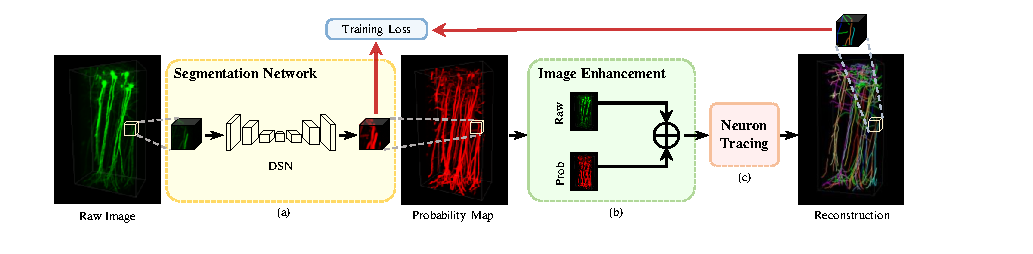
\includegraphics[width=1\textwidth]{./Illustrations/framework_plnpr.pdf}
	\caption{Diagram of our progressive learning algorithm for neuron reconstruction from an image block. (a) The segmentation network extracts neuron signals from the raw image. (b) The output probability map is employed to enhance the raw image in order to preserve both global structures and local signal details, which facilitates the neuron tracing module (c) for more complete neuronal population reconstruction. To train the segmentation network, we use the reconstructed neurons as pseudo labels (red arrows), and iteratively refine the network model and neuron reconstruction with a set of images. The black arrows show the reconstruction pass from an image block at the test stage.}
	\label{fig:framework}
\end{figure*}


Given an ultra-scale noisy OM image, our UltraNPR follows a block-by-block neruon reconstruction scheme, as Fig.~\ref{fig:ultra_framework} shows. 
%
The ultra-scale input image may contain billions or even trillions of voxels.
We first divide the input image into blocks that are averagely in size of $0.5mm\times 1mm\times 0.4mm$ with overlaps. 
%
For each block, we first enhance the noisy images by a deep neural network, which is progressively trained from reconstructed neurons using our PLNPR. 
Then we reconstruct neuronal populations in each block using the enhanced image. 
%
Since it is more reliable to start from somas rather than subtle neurites for neuron reconstruction, we first detect somas and start tracing from the blocks where somas can be detected. 
%
Our UltraNPR then employs an effective block propagation strategy to trace dense neuronal populations in an adaptive order by finding neighboring blocks with more neurite tips. 
Finally, we fuse overlapped neurites in adjacent blocks to reconstruct complete neuronal populations from the whole ultra-scale image.


\subsection{PLNPR for Robust Neuron Reconstruction}
%\subsection{Unsupervised Progressive Learning for Neuronal Population Reconstruction}
\label{sec:PLNPR}

To reconstruct neurons from a noisy OM image block, our PLNPR algorithm consists of three key components: a segmentation network, an image enhancement module, and a neuron tracing module, as shown in Fig.~\ref{fig:framework}. 
%
The segmentation network is designed to extract neuron voxels from noisy and complex backgrounds.
Compared with existing segmentation networks that are trained with dense voxel-wise annotations for strong supervision, we use pseudo labels that are generated using traditional neuron tracing methods.
%
In each iteration of segmentation and reconstruction, we apply the NGPST~\cite{Quan2015} as the neuron tracing module to reconstruct neurons from image blocks. 
The tracing module can be replaced by any other tracing method that does not require manual annotations for training.
%
It takes an image block $\mathbf{B}$ as input and reconstructs a neuronal population with separated neurons.
%The intensity $\mathbf{I}(x)$ of a voxel $x$ belongs to $[0,1]$.
From the reconstruction results, we produce a binary mask $\mathbf{M}$ indicating foreground by $\mathbf{M}(x)=1$ and background by $\mathbf{M}(x)=0$ for a voxel $x$.


Given $N$ unlabeled image blocks, we train our segmentation network using the neuron masks $\{\mathbf{M}_i\}_{i=1}^{N}$ generated from the neuron tracing module.
%
The output of the neuron segmentation network is a 3D probability map $\mathbf{P}$, which is computed by a voxel-wise softmax activation function. $\mathbf{P}(x)\in [0,1]$ indicating the probability of a voxel $x$ to be a neuron part.
%
Then, by fusing the predicted probability map with the raw image signals, the image block is enhanced in order to preserve both local signals and global structures simultaneously.
When the enhanced block is fed into the neuron tracing module, more complete neuronal populations can be reconstructed and provide better pseudo labels for the next iteration of network training. 
%
Based on the iterative learning process, the DNN and neuron tracer mutually complement and promote each other to gradually improve the neuron reconstruction performance.


 

\subsubsection{DNN for 3D Neuron Segmentation}
\label{sec:network}
 
Extracting neuron voxels from image blocks is non-trivial since the size, morphology, and intensity of neurons vary significantly.
In recent years, many 3D DNNs, such as 3D U-Net~\cite{Cicek2016}, 3D DSN~\cite{Dou2017}, and DenseVoxNet~\cite{Yu2017}, have demonstrated their outstanding capability in various biological and biomedical image segmentation tasks.
%
We extend the 3D DSN~\cite{Dou2017} as our neuron segmentation network to balance the performance and computation burden.
%
Although the original 3D DSN has achieved excellent performance for 3D organ segmentation~\cite{Dou2017}, it is prone to overfit in our case due to the limited training data. 
We employ the dropout~\cite{Srivastava2014} technique during training to learn more robust features that better generalize to new data.
In each convolutional layer, the dropout with a rate of $0.5$ is applied.% in our network. 


Another challenge in training 3D DNN is the memory limitation because the 3D feature images are huge with respect to the input size. Therefore, for each input image block, we crop a group of small cubes in size of $160\times 160\times 160$ with $30\%$ overlaps, and set batch size to 1 during training. 
%
To have the same physical resolution with the lateral dimension in OM image blocks, voxels in the axial dimension are interpolated after the imaging process. However, this interpolation leads to inhomogeneous image quality along different dimensions. 
Therefore, a random transposition process is employed for each cube as data augmentation for network training.

%Correspondingly, at the test time, we stitch these overlapped probability cubes together using average blending to get a probability map in the same size with the input block.

In addition, the volume of neuron voxels is usually much smaller than that of background in an OM image.
A data balancing technique is employed for network training.
When computing the training loss, we only consider the neuron voxels and a certain portion of background, which is randomly selected as non-neuron samples.
The number of non-neuron voxels used for training is set as $10$ times that of neuron voxels.


\subsubsection{Image Enhancement}
\label{sec:enhancement}

After training the segmentation network using pseudo labels, the trained model is used to predict a probability map for each image cube. 
By averaging the probabilities of the overlapped voxels between adjacent cubes, we can obtain the probability map $\mathbf{P}$ for the entire block $\mathbf{B}$.
Each element in $\mathbf{P}$ indicates the probability of the corresponding voxel in $\mathbf{B}$ being a neuron voxel.
To utilize the probability map, one natural way is to reconstruct neurons directly from it.
However, since the pseudo labels are not as accurate as manual annotations, especially at the early iterations, some local details might lose in the probability map. Therefore, we employ an enhanced representation by fusing the probability map and the raw image block in order to keep detailed structures and suppress noise signals effectively.
Specifically, a new probability map $\widetilde{\mathbf{P}} $ is first constructed by linearly mapping the value range of $ \mathbf{P}\in [0,1] $ to the value range $[{b}_{min}, {b}_{max}]$ of $\mathbf{B}$ as
\begin{equation}
\widetilde{\mathbf{P}}(x) = ({b}_{max}-{b}_{min})\mathbf{P}(x).
\end{equation}
%
Then, an enhanced block $\mathbf{E}$ is computed as
\begin{equation}
\mathbf{E}(x) = \alpha\widetilde{\mathbf{P}}(x) + (1-\alpha)\mathbf{B}(x),
\label{equ: enhance}
\end{equation}
where $\alpha\in [0,1]$ is a weight to control the contributions of voxel $ x $ in the original intensity and the probability map. By feeding the enhanced block to the neuron tracing module, neuronal populations can be reconstructed more completely.


With more reliable reconstruction results as pseudo labels, the segmentation network could be further trained to learn more discriminative and representative features for producing probability maps, which in turn benefit the tracing module to reconstruct more complete neurons in the next iteration.
%
As shown in Fig.~\ref{fig:ngps} (a), a raw image block typically contains many noises and inhomogeneous intensities.
At first, by feeding the raw block to the tracer~\cite{Quan2015}, the reconstructed neuronal population is incomplete and many neurites are missing, as Fig.~\ref{fig:ngps}(g) shows, comparing with the ground truth (GT) shown in Fig.~\ref{fig:ngps}(k).
%
Then, by utilizing the pseudo labels derived from imperfect reconstruction, the segmentation network can be trained to learn features for global morphology. Fig.~\ref{fig:ngps}(b) shows the predicted probability map, which demonstrates the enhanced trajectories.
With more iterations of neuron reconstruction and network training, more distinctive and long-range trajectory features can be progressively captured by the network, as shown in Fig.~\ref{fig:ngps}(c)(d)(e).
By combining the original image intensities with the predicted probability map, both local signal details and global trajectories are well preserved in the enhanced block, as Fig.~\ref{fig:ngps}(f) shows.
Iteration by iteration, the completeness and accuracy of neuron reconstruction are progressively improved, as shown in Fig.~\ref{fig:ngps}~(h)(i)(j).


\begin{figure}[t]
	\centering
	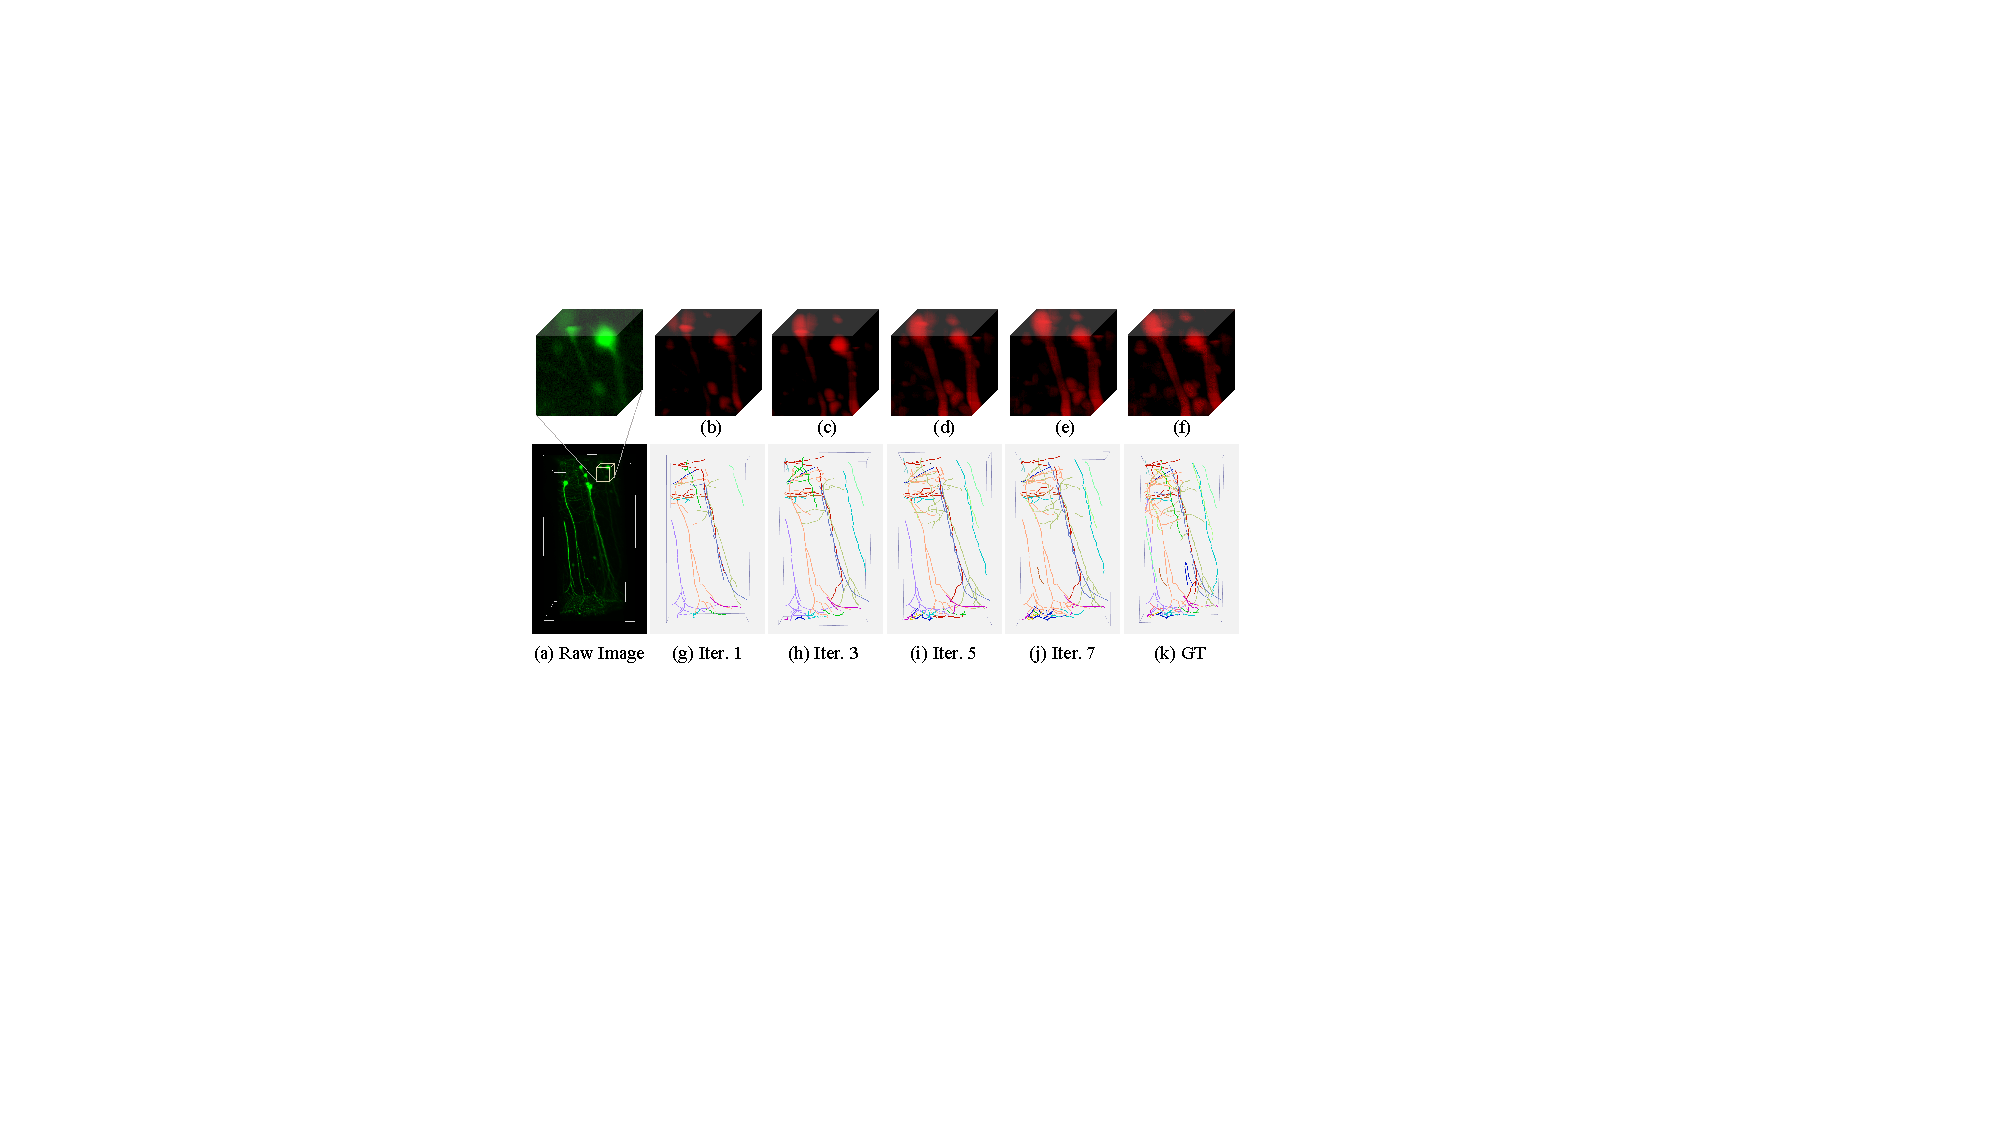
\includegraphics[width=1\columnwidth]{./Illustrations/ngps.pdf}
	\caption{Our progressive learning technique gradually improves the segmentation network to extract neuron signals from a raw image block (a). 
	(b-f) The probability maps generated by the segmentation network at different iterations.
		%Combing the probability map and the raw intensity, the enhanced block preserves both global trajectory and local details. 
	(g-j) More and more complete and accurate reconstruction of the neuronal populations can be obtained with more iterations. (k) Manually labeled neurons. Separated neurons are shown in different colors.}
	\label{fig:ngps}
\end{figure}
%

\subsection{Ultra-scale Neuronal Population Reconstruction}
\label{sec:UltraNPR}

\begin{figure}[t]
	\centering
	%\vspace{1cm}
	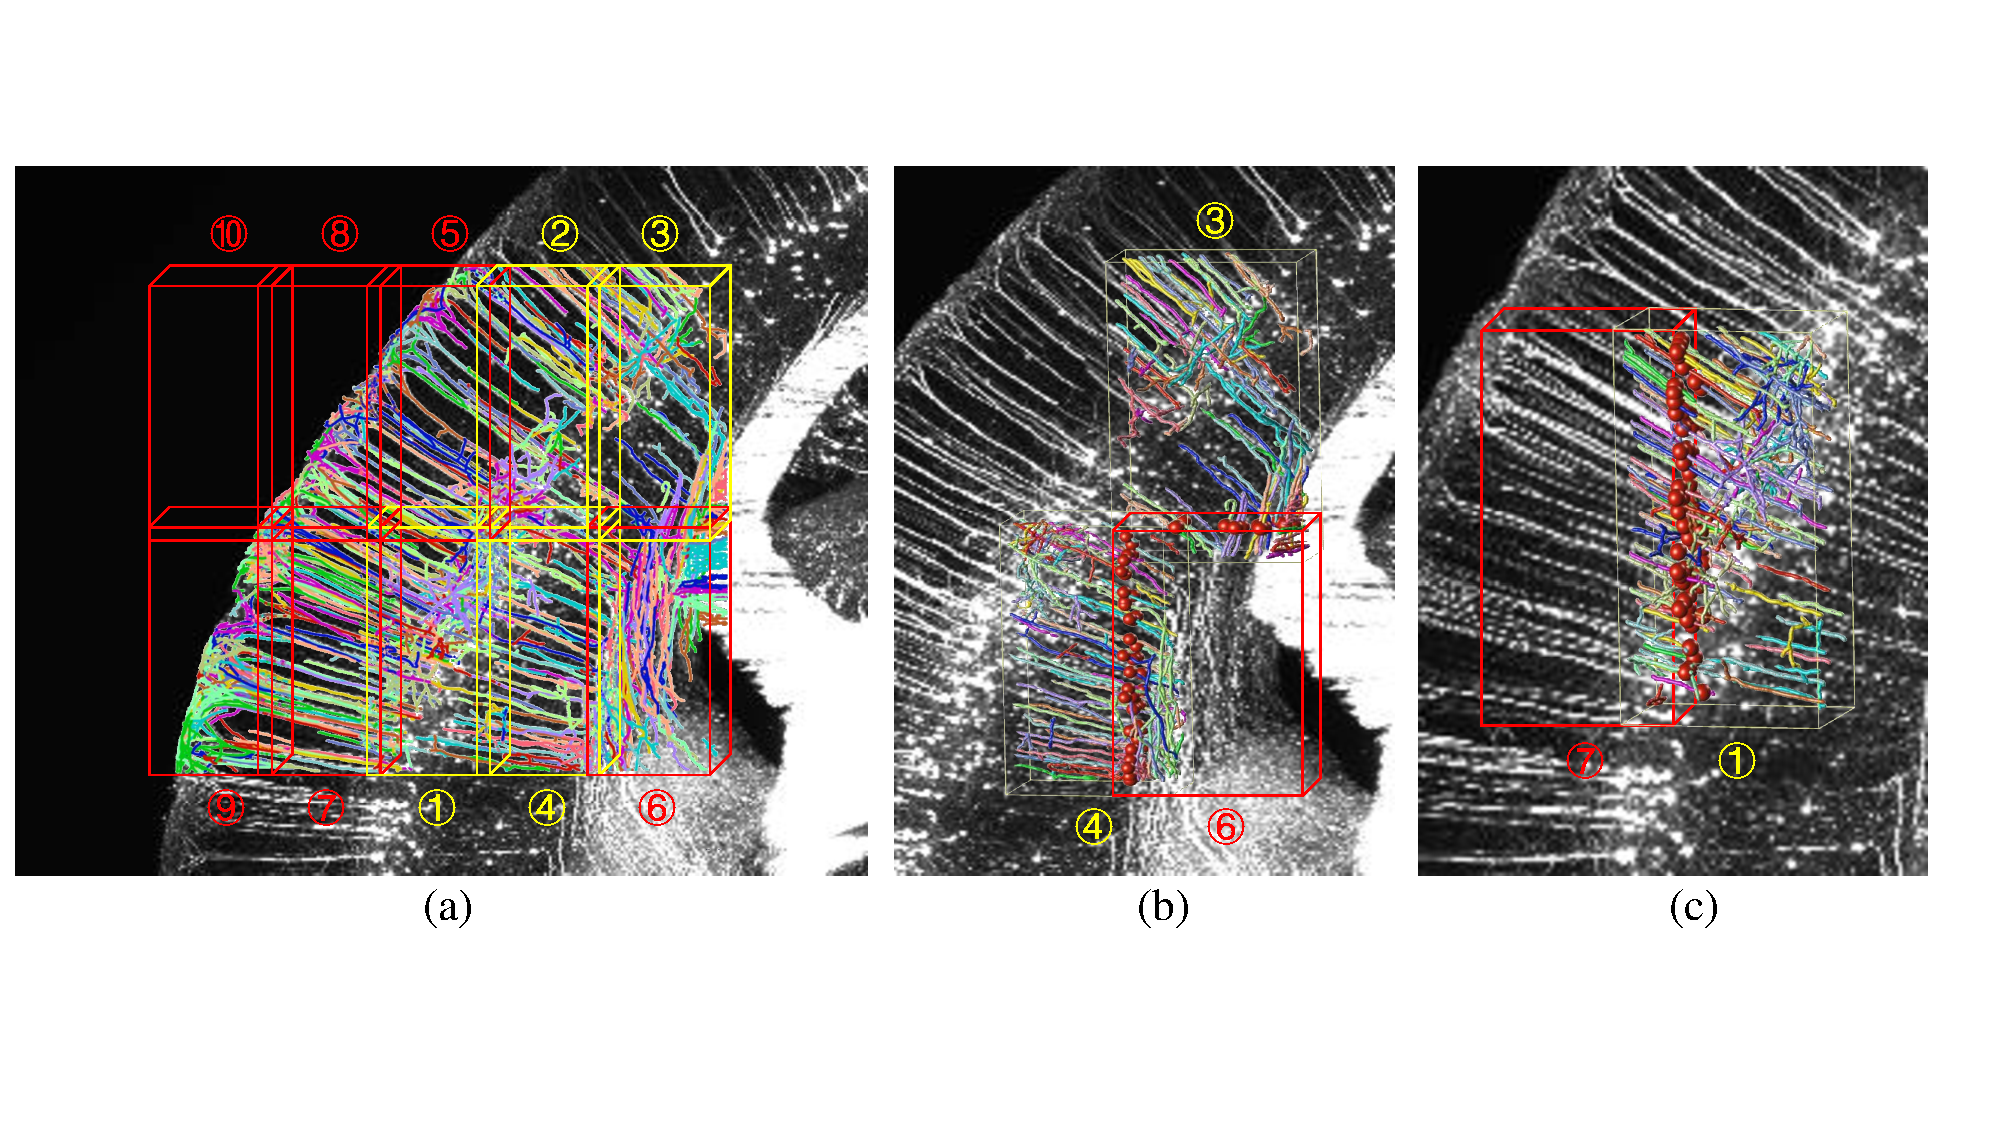
\includegraphics[width=1\columnwidth]{./Illustrations/ultranpr_block_search.pdf}
	\caption{An example of the iterative block reconstruction for ten blocks. (a) The number indicate the order in which the ten blocks are traced. The blocks 1, 2, 3, 4 are firstly reconstructed using our PLNPR since there are somas detected in these four blocks. (b) Block-6 is reconstructed by setting the neurite tips (red dots) from its two neighboring blocks (3, 4) as pseudo somas for tracing. (c) Block-7 is reconstructed by setting the neurite tips from its neighboring block-1 as pseudo somas.}
	\label{fig:blocksearch}
\end{figure}


Our PLNPR enhances the image signals and traces neurons from each image block.
However, neurons usually exist across multiple blocks in an ultra-scale image. 
% 
We propose an effective stitching process by looking for the most continuous block to trace dense neuron populations from all unreconstructed blocks. 
%
As somas are where signals from the dendrites are joined and pass on, we start from reconstructing neurons in the blocks where somas can be detected.
For blocks where no soma can be detected, we trace the neurons by generating pseudo-somas from the neurite tips of their neighboring blocks. 
%
Finally, the overlapped neurites reconstructed from adjacent blocks are fused to get a complete reconstruction of neurons. 
Fig.~\ref{fig:ultra_framework} shows the pipeline of our UltraNPR approach. 
%Our UltraNPR consists of four components: a soma detection module, a block reconstruction module, a block search module, and a neurite fusion module, as shown in

\delete{
%\subsubsection{Initial Soma Detection}
%\label{sec:soma}
 %
 %For each block $B_{i}$, we get a set of somas.
 % $\hat{S}_i = s_{ik}, k=1,\ldots,M_{i} $. 
 %Each soma $ s_{ik} $ is represented by its center $ (x,y,z) $ and radius $ r $.
We apply the soma detection algorithm~\cite{Quan2013} on each block in an ultra-scale image separately. 
Due to the overlap between blocks, somas in the overlapped area would be detected repeatedly.
We merge the overlapping somas in adjacent blocks by averaging their positions and radius and get a set of somas in the entire image, \md{as shown in Fig.~4 of the supplementary file.} 
%The soma detection results from the large-scale image are visualized in Fig.~{4} of the supplementary file.
%These somas are also used to define the initial blocks for neuron reconstruction in the next step.
}

\subsubsection{Block Reconstruction and Propagation}
\label{sec:trace}


 
We apply the soma detection algorithm~\cite{Quan2013} on each block in an ultra-scale image separately. 
If a block $B_{i}$ contains somas, we apply our PLNPR to reconctruct neurites and get a set of neurites $\mathcal{N}_{i}$ in this block, as shown by the blocks in yellow frames in Fig.~\ref{fig:blocksearch}~(a).
The reconstruction result of each neurite is saved as an SWC file~\cite{Cannon1998}, a text file that consists of a series of dense neuron points containing an index, radius, type, and connectivity information.
% As a neuron reconstruction produced by our method is represented by a series of voxel-vise dense reconstruction compartments that have different coordinates and radius, 
%For the remaining unreconstructed blocks, we check its neighboring blocks that have been reconstructed and add the neurite tips from the reconstructed blocks as its pseudo somas. 
%
For the remaining unreconstructed blocks, though NGPST can perform neuron tracing without any somas, it typically fails to distinguish multiple neurons with dense neurites, as shown in Fig.~\ref{fig:ngpst_pseudosoma}~(a).
%
In order to avoid under-segmentation of neurons in an unreconstructed block $B_u$, we follow the neuron structure in its neighboring blocks that have been reconstructed.
%
More specifically, for each neighboring reconstructed block of $B_u$, we collect the neuron points that intersect the boundary of $B_u$ and use them as the pseudo-somas for growing the neuronal structure in $B_u$, as shown in Fig.~\ref{fig:blocksearch}~(b)(c). After that, we get the neurites set $ \mathcal{N}_u$ in $B_u$.
%
Therefore, for each iteration of our block propagation, the unreconstructed block which has the largest number of neighboring reconstructed blocks and the largest number of pseudo somas is selected for reconstruction next.
%
Fig.~\ref{fig:blocksearch} shows the block propagation and reconstruction process of ten neighboring blocks. 
%(b)(c) show two examples of unreconstructed blocks (red) that to be traced from its neighboring blocks (yellow) that have been reconstructed. 
%
This process continues iteratively until all the blocks in the ultra-scale image have been reconstructed. 
%
%\md{Fig.~\ref{fig:blocksearch} shows the procedure of our iterative local reconstruction. the order of propagation, comparison between NGPST with/without neurite tips as pseudo somas. }

\begin{figure}[t]
	\centering
	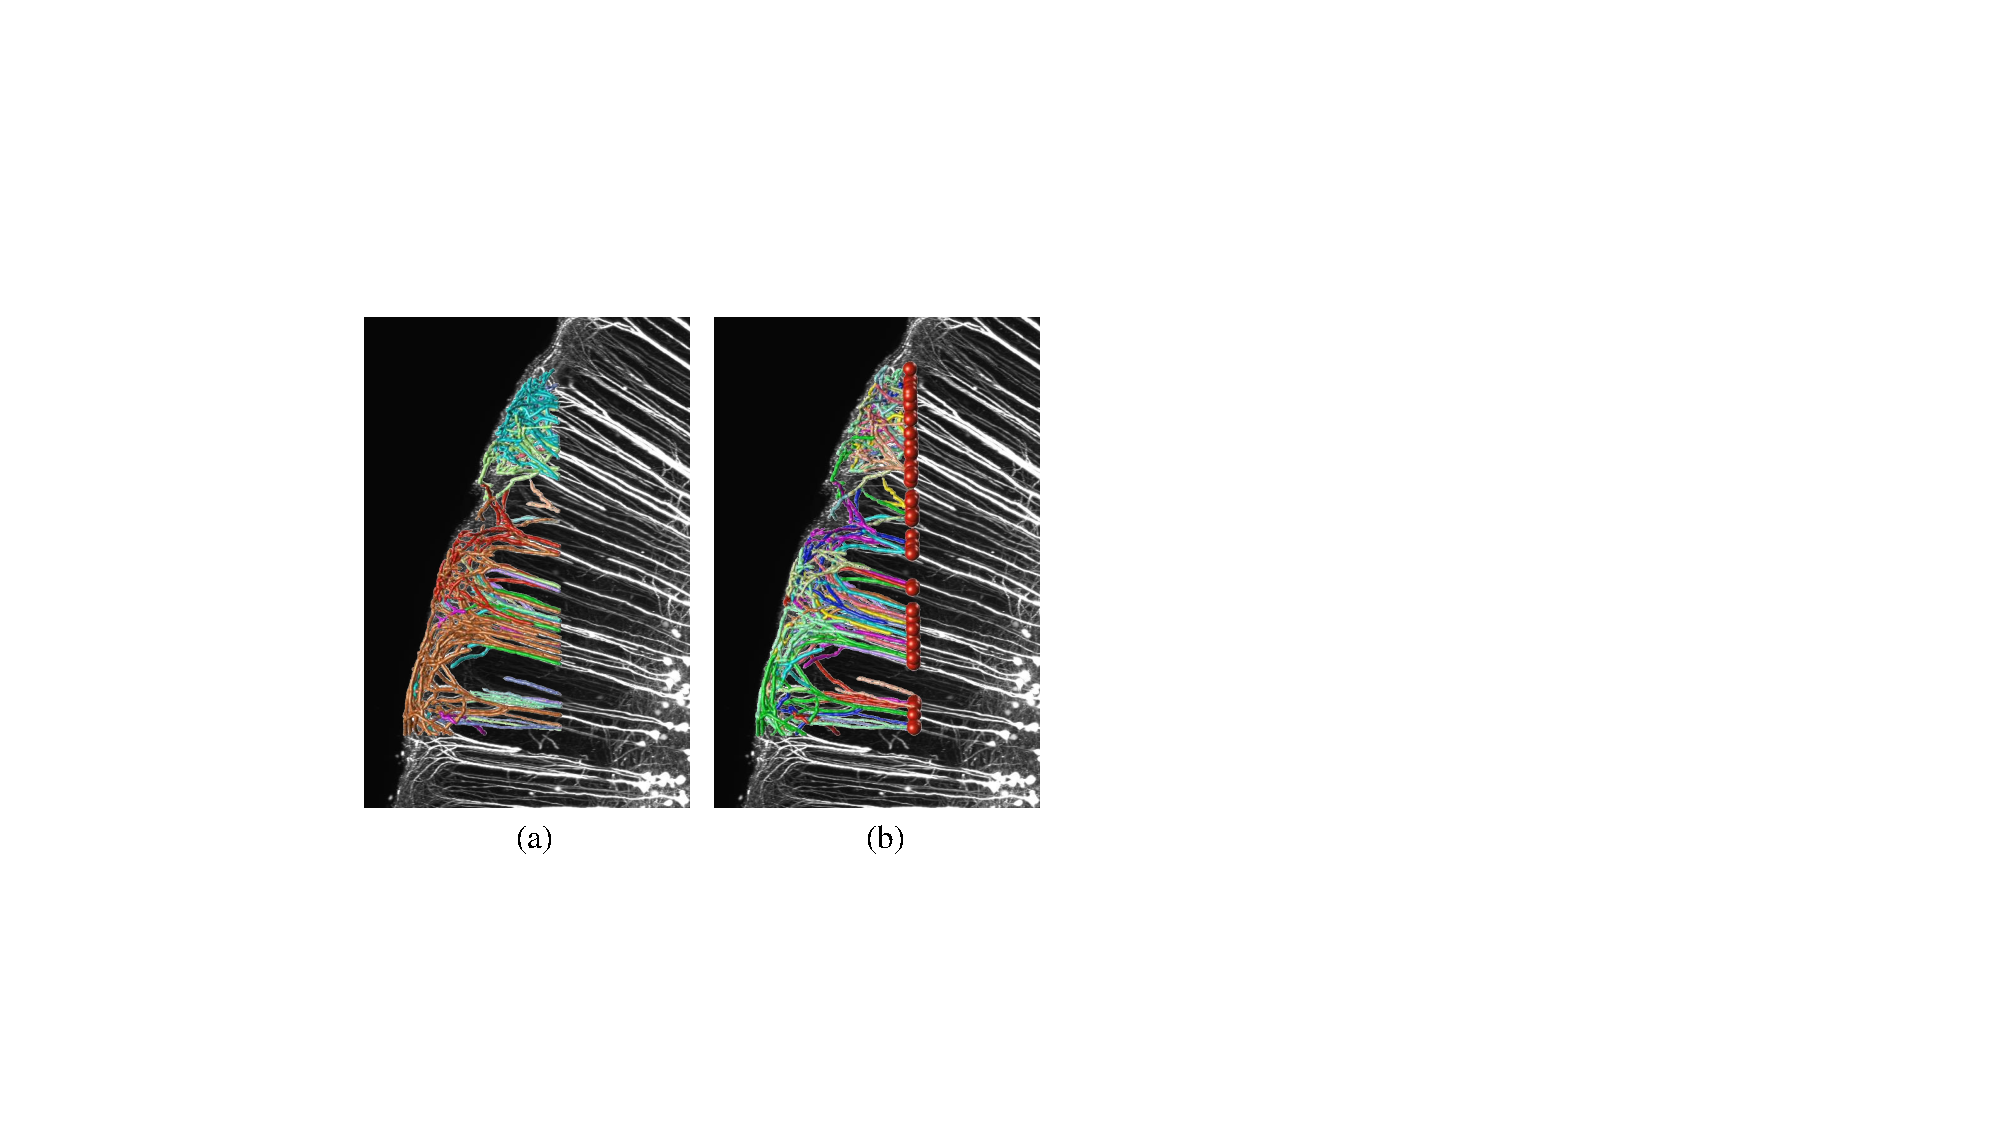
\includegraphics[width=0.85\columnwidth]{./Illustrations/ngpst_pseudosoma.pdf}
	\caption{Comparison of neuron reconstruction results from an enhanced image block by NGPST without setting somas (a) and setting neurite tips (red points) from a neighboring block as pseudo somas (b). Separated neurons are shown in different colors.}
	\label{fig:ngpst_pseudosoma}
\end{figure}



\subsubsection{Neurite Fusion in Adjacent Blocks}
\label{sec:fusion}


\begin{figure}[b]
	\centering
	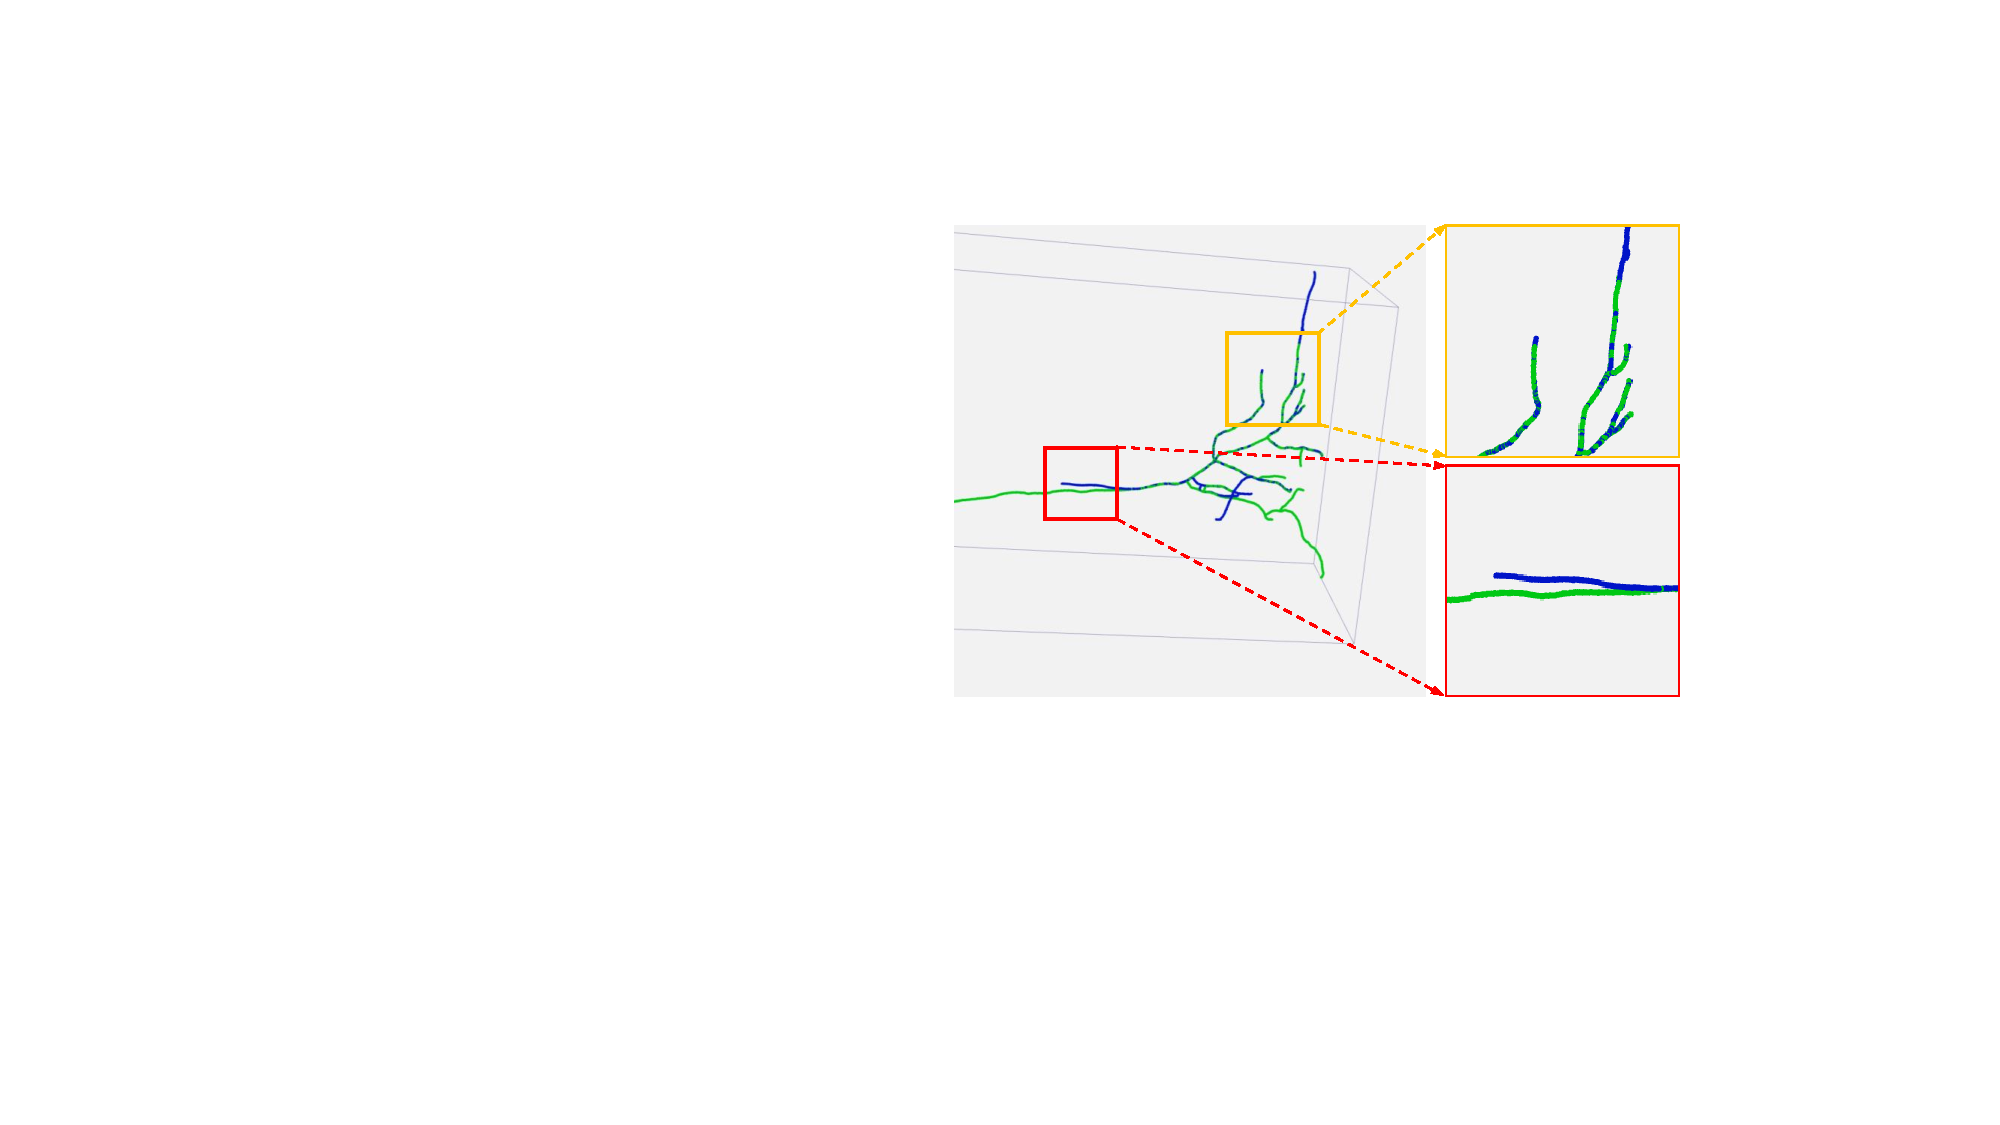
\includegraphics[width=0.86\columnwidth]{./Illustrations/fusion_errors.pdf}
	\caption{An example of over-tracing (yellow) and topological discrepancy (red) when assembling two overlapped neurites. These reconstructions are shown in skeleton mode for better visualization.}
	\label{fig:overlap_discrepancy}
\end{figure}
Since neurons would be split into fragmented neurites when dividing the raw image into blocks, we now fuse the neurites reconstructed separately from adjacent blocks into individual and complete neurons.
Given the reconstructed neurite sets $\mathcal{N}_a$ and $\mathcal{N}_b$ in two overlapped blocks $\mathbf{B}_a$ and $\mathbf{B}_b$ respectively, for any pair of neurites $N_a$ and $N_b$ in the two sets respectively, if their overlapping volume is larger than a threshold $\delta_{ovlp}$, we fuse them together to get a more complete neurite.

There might be over-tracing and topological discrepancy between two neurites that are reconstructed in two blocks separately, as shown in Fig.~\ref{fig:overlap_discrepancy}.
Generally, the reconstruction quality near the block boundary is less accurate and reliable than that in the middle of blocks because of less context. 
Therefore, when fusing two neurites, we tend to keep the neurite segments in the middle of blocks as following.
%But this region is inside the adjacent block due to the overlap between them, which means substantial context information of this region can be provided to the tracing methods and leads to a better reconstruction.
%Therefore, when assembling two matched neurites from adjacent blocks, we only consider neuronal \md{points} which are not near the boundary of the corresponding block. 
  
To fuse two neurites, we first select the longer one as the reference neurite $N_a$, and fuse the other neurite $N_b$ to the reference neurite, as shown in Fig.~\ref{fig:fusion_algorithm} (b).
%
Each neurite is decomposed to a set of neurite branches, as Fig.~\ref{fig:fusion_algorithm} (c) shows.
Each branch is sampled uniformly into a set of neuron compartments, as Fig.~\ref{fig:fusion_algorithm} (d) shows.
%
For each branch $\brc_b$ of neurite $N_b$, we search the branch $\brc_a$ of $N_a$ which has the largest overlapped volume with $\brc_b$, as Fig~\ref{fig:fusion_algorithm} (f) shows.

To fuse the matched two branches, for each point $p_a$ in the branch $\brc_a$, if $p_a$ lies in the boundary region of block $\blk_a$ ($\delta_{bound}$ voxels to the block boundary of $\blk_a$), it will be removed and all its child branches are also deleted, as shown in Fig~\ref{fig:fusion_algorithm} (g).  
The same deletion operation is performed on the points in the branch $\brc_b$ that are located in the boundary regions of block $\blk_b$.
%
Then, for each remaining point $p_b$ in branch $\brc_b$, if there is a point $p_a$ in branch $\brc_a$ so that $dis(p_b,p_a)<\delta_{pt}$, it will be removed since the point $p_a$ is kept, as Fig~\ref{fig:fusion_algorithm} (g) shows.
%
After that, the remaining part of branch $\brc_b$ is merged to the reference branch $\brc_a$ by connecting it to the nearest point in $\brc_a$.
After all matched branches are processed as above, we can obtain the fused neurite $N_{ab}$.
%
For the remaining branches in $N_b$ which are not fused to any branches in $N_a$, they will be merged to the neurite $N_{ab}$ by connecting each of them to the nearest point in $N_{ab}$.
%
Fig~\ref{fig:fusion_algorithm} (h) shows the final fusion result of the two neurites. 
By fusing all neurites in two adjacent blocks, we can obtain more complete reconstruction of dense neuronal populations, as shown in Fig~\ref{fig:fusion_algorithm} (e).


 
 \begin{figure}[t]
 	\centering
 	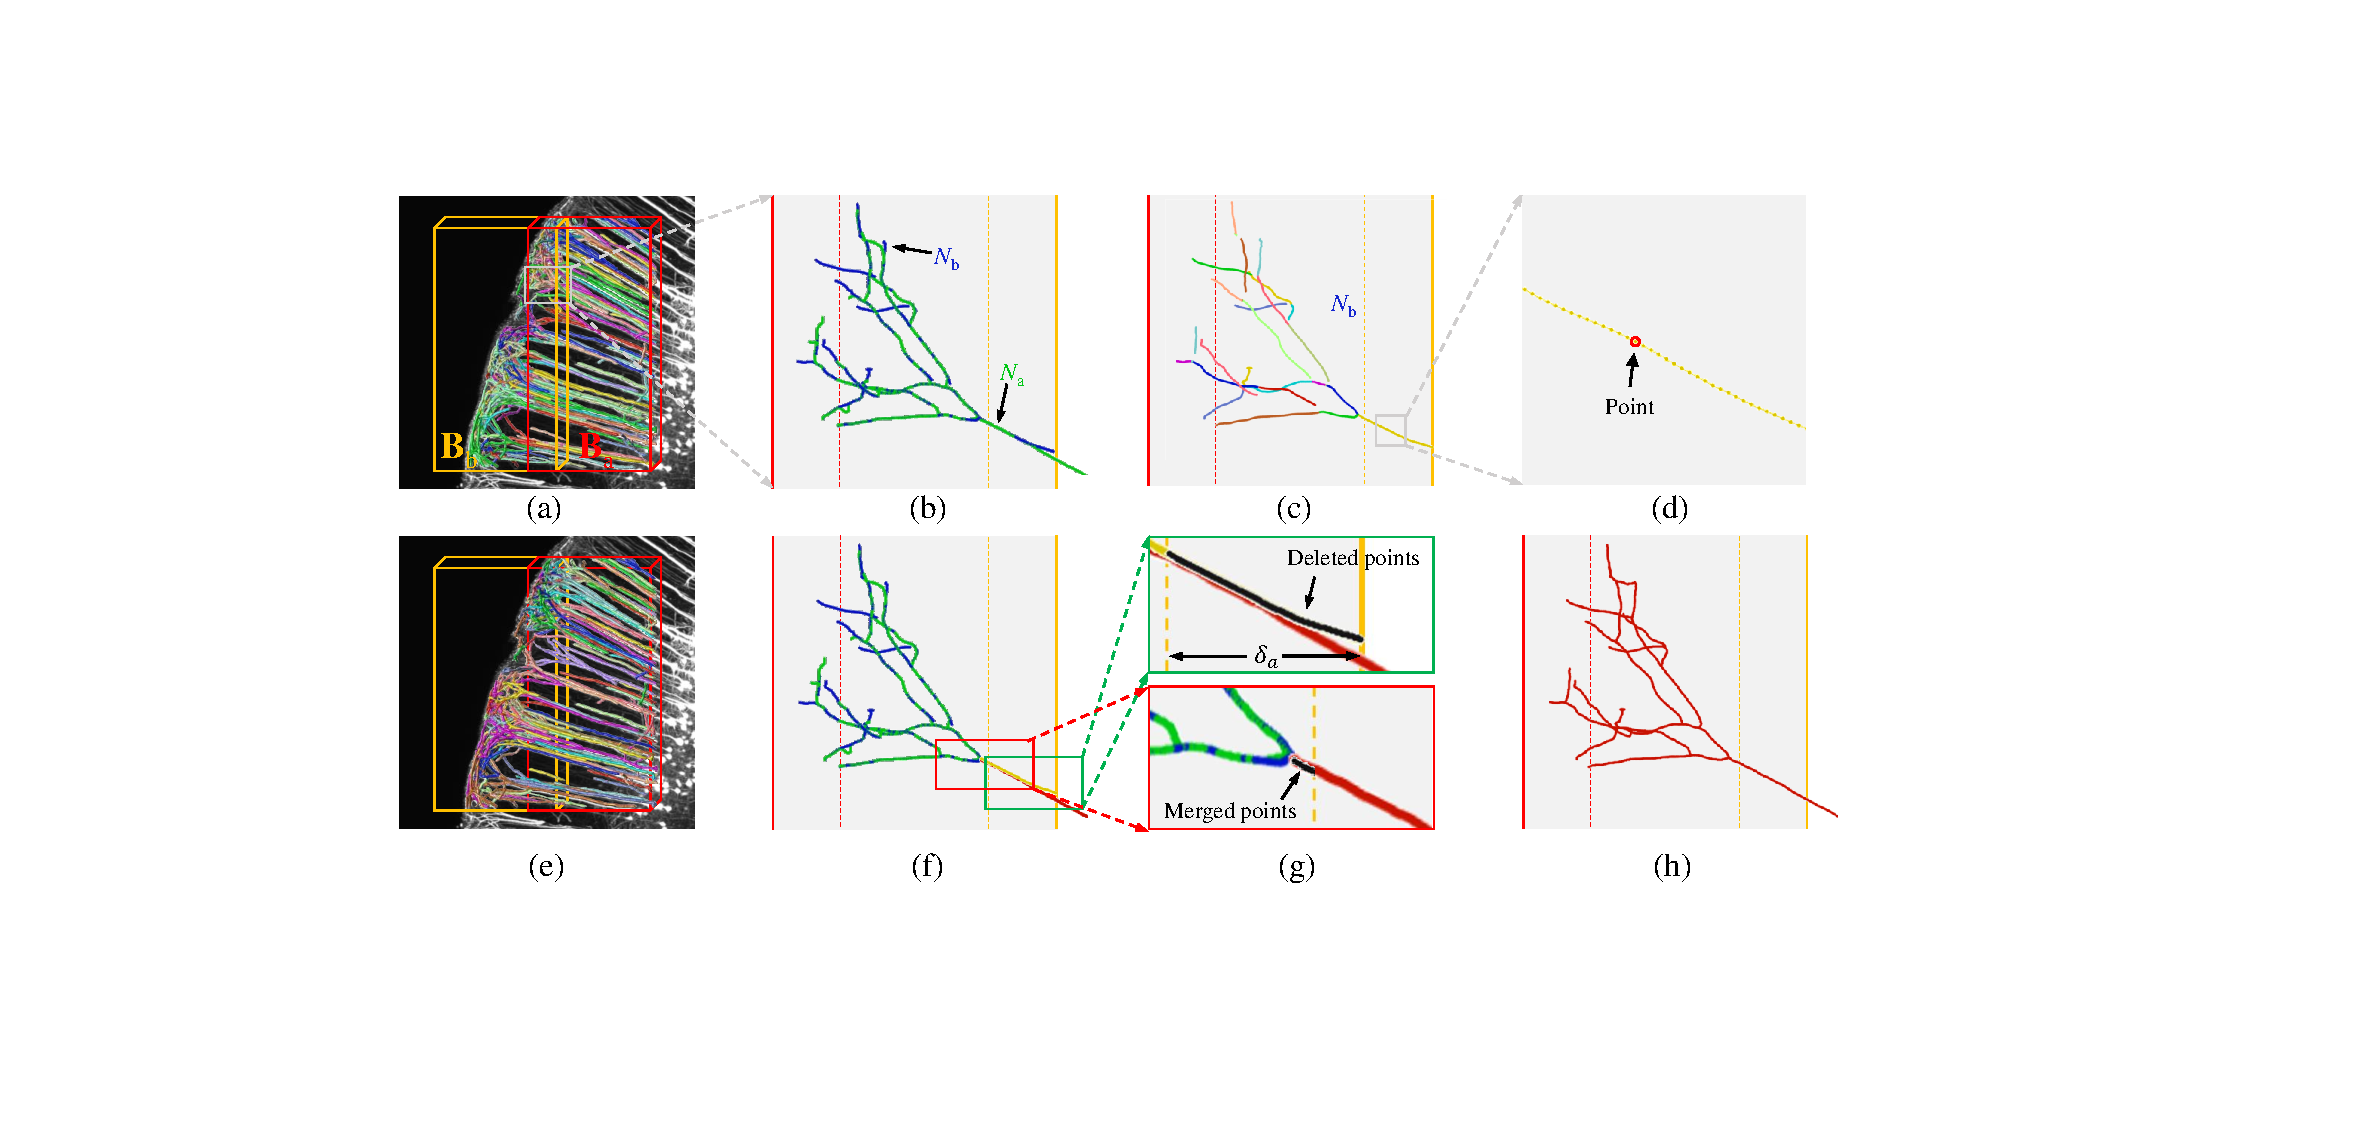
\includegraphics[width=1\columnwidth]{./Illustrations/fusion_algorithm.pdf}
 	\caption{Neurite fusion in two adjacent blocks. (a) Neurites reconstructed separately in two blocks. For two matched neurites $N_a$ and $N_b$ (b), each neurite is decomposed to branches (c) and each branch is sampled into points (d). We delete the points in the boundary regions and merge the points in the middle area of the block (g) to get a more smooth and complete neurite (h). (e) Fusion results of two blocks. }
 	\label{fig:fusion_algorithm}
 \end{figure}
 
 


